\documentclass[conference]{IEEEtran}
\IEEEoverridecommandlockouts
\usepackage[utf8]{inputenc}
\usepackage[spanish,es-tabla,es-noshorthands]{babel}
\usepackage{cite}
\usepackage{amsmath,amssymb,amsfonts}
\usepackage{graphicx}
\usepackage{xcolor}
\usepackage{hyperref}
\usepackage{booktabs}
\usepackage{tabularx}
\usepackage{makecell}
\usepackage{pifont}
\usepackage{array}
\usepackage{listings}
\usepackage{float}
\usepackage{geometry}
\usepackage{placeins}
\usepackage{tikz}
\usetikzlibrary{shapes.geometric, shapes.multipart, arrows.meta, positioning, calc, fit, backgrounds, decorations.pathreplacing, patterns}

\graphicspath{{figures/}}

\geometry{
  letterpaper,
  top=2.5cm, bottom=2.5cm,
  left=2.5cm, right=2.5cm
}
\onecolumn

\hypersetup{
  colorlinks=true,
  linkcolor=blue!50!black,
  citecolor=blue!50!black,
  urlcolor=blue!60!black
}

\renewcommand{\topfraction}{0.9}
\renewcommand{\bottomfraction}{0.8}
\renewcommand{\textfraction}{0.1}
\renewcommand{\floatpagefraction}{0.7}

\lstdefinelanguage{json}{
  morestring=[b]",
  stringstyle=\color{teal!70!black},
  showstringspaces=false,
  breaklines=true,
}
\lstdefinelanguage{yaml}{
  keywords={true,false,null,enabled,replicas,size,name},
  keywordstyle=\color{blue!70!black}\bfseries,
  sensitive=false,
  comment=[l]{\#},
  commentstyle=\color{gray}\itshape,
  morestring=[b]',
  stringstyle=\color{teal!70!black},
  breaklines=true,
}

\lstset{
  basicstyle=\ttfamily\scriptsize,
  breaklines=true,
  frame=single,
  framerule=0.4pt,
  rulecolor=\color{gray!50},
  commentstyle=\color{gray!80!black},
  keywordstyle=\color{blue!70!black}\bfseries,
  numbers=left,
  numberstyle=\tiny\color{gray},
  xleftmargin=1.2em,
  framexleftmargin=1.2em,
  showstringspaces=false,
}

\begin{document}

\title{Plataforma distribuida en la nube para la detección anticipada del Síndrome de Visión por Computador a partir de telemetría conductual}


\author{
  \IEEEauthorblockN{Andersson D. Sánchez Méndez,
                    Cristian S. Pedraza Rodríguez,
                    Jeisson D. Sánchez Gómez}
  \IEEEauthorblockA{Programa de Ingeniería de Sistemas,
                    Escuela Colombiana de Ingeniería Julio Garavito\\
                    Bogotá D.C., Colombia\\
                    \{andersson.sanchez-m, cristian.pedraza-r,
                    jeisson.sanchez-g\}@mail.escuelaing.edu.co}
}

\maketitle

\begin{abstract}
Después de la pandemia, trabajar varias horas al día frente a un computador
se volvió la norma en oficinas y en trabajo remoto. Esa exposición continua
está asociada al Síndrome de Visión por Computador (CVS), que reúne
síntomas oculares y musculoesqueléticos y afecta a un porcentaje alto
de quienes pasan más de cuatro horas con pantallas. Las herramientas que
hoy se usan para mitigarlo (Apple Screen Time, Google Digital Wellbeing,
f.lux) viven en el dispositivo y solo cuentan tiempo: no comparten
información entre usuarios ni le dan visibilidad a un área de salud
ocupacional.

Este trabajo describe el diseño y la implementación parcial de una
plataforma distribuida que toma tres señales del celular (luz ambiente,
distancia al rostro y tiempo activo de pantalla), las manda a la nube y
calcula un puntaje de riesgo de CVS por usuario, con un tablero agregado
por área. El prototipo está construido sobre Kafka, InfluxDB y un modelo
XGBoost entrenado con un dataset sintético de 50.000 registros, ya que
conseguir datos clínicos reales no era viable en el alcance del semestre. 

Sobre ese dataset el clasificador alcanza un F1 macro de
0{,}85 y un AUC-ROC de 0{,}89, y una auditoría automatizada con cinco
pruebas verifica que ningún identificador crudo llega a la base de datos.
La validación clínica con un grupo de trabajadores reales queda como
trabajo futuro.
\end{abstract}

\begin{IEEEkeywords}
Síndrome de visión por computador, telemetría conductual, arquitectura
distribuida, Kafka, InfluxDB, aprendizaje automático, salud ocupacional.
\end{IEEEkeywords}

\section{Contexto}

Trabajar frente a un computador dejó de ser una actividad puntual y se
volvió la forma básica de trabajar en el sector servicios. En Colombia, 
la jornada típica del sector tecnología son entre ocho y diez horas 
continuas frente a un monitor, sin contar el celular. Eso ya da entre 40 
y 50 horas semanales solo de pantalla de trabajo, antes de sumar el uso 
personal del teléfono fuera de oficina.

El mecanismo fisiológico es simple y está medido. Una persona en reposo 
parpadea entre 15 y 20 veces por minuto; concentrada leyendo en pantalla, 
baja a 4 o 6. Con menos parpadeos la película lagrimal se rompe, y de ahí 
salen los síntomas que cualquiera que haya trabajado un día largo conoce: 
ojos secos, ardor, visión borrosa, dolor de cabeza \cite{sheppard2018}. 
Eso es el Síndrome de Visión por Computador (CVS), o Digital Eye Strain, 
y los estudios reportan prevalencias de entre el 50\,\% y el 90\,\% según 
el país y los criterios usados \cite{sheppard2018}.

Desde el lado de la empresa, esto es plata: un trabajador con CVS produce 
menos. La Asociación Americana de Optometría estimó pérdidas de
productividad por fatiga visual del orden de decenas de miles de millones 
de dólares al año en Estados Unidos \cite{aoa2023}. Por eso varias áreas 
de salud ocupacional ya lo están tratando como riesgo medible y no como 
una molestia individual más.

Una cuenta rápida nos sirvió para aterrizar el orden de magnitud local. 
Para una empresa de 1.000 trabajadores en Bogotá, asumiendo prevalencia 
del 69\,\%, una pérdida promedio del 18\,\% en productividad y un salario 
profesional medio de USD~18.000 al año, el costo anual atribuible a CVS 
no manejado es del orden de USD~2,3 millones. Los porcentajes son 
discutibles, pero el orden de magnitud ya saca la conversación del 
bienestar individual y la mete en salud ocupacional.

Lo que existe hoy para mitigar el CVS son apps de bienestar digital: Apple 
Screen Time, Google Digital Wellbeing, f.lux. Todas hacen básicamente lo 
mismo: cuentan minutos en pantalla, y cuando se pasa un umbral fijo 
muestran una notificación. No miran si la luz del puesto es mala, ni si 
el usuario está muy cerca del monitor, ni si lleva tres horas sin parar. 
Y, lo que para nosotros era el punto, no le sirven al área de salud 
ocupacional de una empresa, porque los datos nunca salen del celular.

\section{Problema}

El problema concreto es este: un área de salud ocupacional, hoy, no tiene 
cómo responder con datos preguntas básicas sobre fatiga visual en su 
empresa. Cosas como cuáles equipos están peor y deberían recibir 
intervención primero, si las pausas activas que la empresa promueve 
sirven o solo generan notificaciones que nadie atiende, o si cuando 
alguien reporta dolor de ojos había señales semanas antes que se 
podrían haber visto.

Para responderlas, los datos tienen que salir del dispositivo, llegar
a un servidor central, integrarse con una identidad organizacional, ser
agregados sin exponer al individuo y procesarse con un modelo que pueda
estimar riesgo. Ninguna pieza por sí sola es nueva; lo que falta es
tenerlas funcionando juntas para este problema en particular.

La brecha que queremos cerrar es entonces de integración: existen 
sensores en los celulares, existen plataformas de mensajería para mover 
telemetría a escala, existen bases de datos de series de tiempo, existen 
modelos de aprendizaje automático livianos, y existe regulación sobre 
datos personales. El reto es ensamblar todo eso en una arquitectura que 
sea defendible técnicamente, que respete la privacidad por diseño y que 
un equipo pequeño pueda construir, desplegar y medir en el alcance de 
un semestre.

\section{Estado del arte}

Lo que ya existe sobre este problema se puede ordenar en tres líneas.

\subsubsection*{Apps de bienestar digital en el dispositivo}

Apple Screen Time, Google Digital Wellbeing y f.lux son las que la gente 
conoce. Todas siguen el mismo patrón: contadores locales con umbrales 
fijos, notificaciones cuando uno se pasa del límite, y los datos nunca 
salen del teléfono. Ninguna expone una API para que un servidor central 
las consulte, ninguna integra señales de contexto como la luz del puesto 
o la distancia al monitor, y ninguna aprende de la población de usuarios. 
Como herramientas de auto-conciencia funcionan; como insumo para un área 
de salud ocupacional, no. La tabla~\ref{tab:vs} resume esta diferencia 
frente a las otras familias de soluciones y frente a nuestra propuesta.

\begin{table}[H]
  \centering
  \small
  \caption{Comparación capacidad por capacidad. \ding{51}\ presente,
    \ding{55}\ ausente.}
  \label{tab:vs}
  \renewcommand{\arraystretch}{1.15}
  \begin{tabular}{@{} l c c c c @{}}
    \toprule
    & \makecell{Bienestar\\digital local} &
      \makecell{Detector\\por cámara} &
      \makecell{Salud IoT\\genérica} &
      \makecell{\bfseries Esta\\\bfseries propuesta} \\
    \midrule
    Telemetría a la nube         & \ding{55} & \ding{55} & \ding{51} & \ding{51} \\
    Sensado no invasivo          & \ding{51} & \ding{55} & \ding{51} & \ding{51} \\
    Modelo entrenado con datos   & \ding{55} & \ding{51} & \ding{55} & \ding{51} \\
    Tablero agregado por área    & \ding{55} & \ding{55} & \ding{51} & \ding{51} \\
    Privacidad por diseño        & \ding{55} & \ding{55} & \ding{55} & \ding{51} \\
    Enfoque específico en CVS    & \ding{51} & \ding{51} & \ding{55} & \ding{51} \\
    \bottomrule
  \end{tabular}
\end{table}

\subsubsection*{Detección por cámara y sensores no visuales}

La línea más explorada en investigación es usar la cámara frontal para 
medir la frecuencia de parpadeo en tiempo real, normalmente con redes 
convolucionales. Funciona, pero tiene dos problemas que para nosotros 
eran bloqueantes: gasta batería y dispara una alarma de privacidad 
inmediata. En una encuesta informal que hicimos en el primer tercio del 
semestre a unos 30 compañeros de la universidad, ``activar la cámara 
para medir si te cansa la vista'' generó rechazo casi unánime, mientras 
que ``leer el sensor de luz del celular'' nadie lo sintió invasivo. Esa 
fue la razón concreta por la que descartamos video y nos fuimos por 
sensores no visuales.

Sobre ese camino sí hay base. El survey de Lane et~al.~\cite{lane2010} 
sigue siendo la referencia estándar para usar acelerómetro, luz ambiente 
y proximidad del celular como proxies de estado del usuario. De ahí 
salen los tres sensores que usamos. Sobre el clasificador, Chen y 
Guestrin~\cite{xgboost} mostraron que XGBoost se comporta muy bien en 
datos tabulares con pocas variables, que es exactamente nuestro caso 
(nueve columnas agregadas). Por eso lo escogimos en lugar de una red 
neuronal, que con tan pocas variables habría sido sobredimensionar.

\subsubsection*{Plataforma y privacidad}

Del lado de infraestructura, el patrón publish/subscribe con un broker 
y una base de serie de tiempo es lo más común para telemetría IoT. 
Kafka~\cite{kafka} para el transporte e InfluxDB~\cite{influxdata} para 
la persistencia son tecnologías con documentación abundante y casos de 
uso ampliamente reportados, lo que nos pareció más sensato que 
experimentar con algo nuevo en un semestre.

Para privacidad nos basamos en el trabajo de Dwork y 
Roth~\cite{dwork2014} sobre privacidad diferencial. Aplicamos dos 
mecanismos: seudonimización del identificador del dispositivo mediante 
HMAC, y ruido aleatorio con distribución de Laplace sobre las lecturas 
continuas antes de persistirlas. El aprendizaje federado de McMahan 
et~al.~\cite{mcmahan2017} es una alternativa interesante para entrenar 
sin centralizar datos, pero su implementación queda fuera del alcance 
del proyecto.

\medskip

No encontramos un sistema que junte estos tres frentes: sensores no 
visuales en el celular, transporte por broker, base de serie de tiempo, 
puntaje de riesgo por usuario, todo aplicado al CVS y con privacidad 
considerada desde el diseño. Ese es el hueco que cubrimos.

\section{Contribuciones}

Lo que aportamos con este trabajo son cuatro piezas.

Primero, una arquitectura distribuida que toma tres señales no invasivas 
del celular del trabajador (luz ambiente, proximidad al rostro y tiempo 
de pantalla activo), las transporta hasta un broker en la nube y las 
procesa con microservicios independientes hasta producir un puntaje de 
riesgo de CVS.

Segundo, un prototipo funcional que corre de punta a punta sobre 
docker compose, con los cuatro microservicios (rule engine, normalizer, 
anonymizer e inference) implementados y orquestados, el agente Android 
en Kotlin, los servicios en Python con FastAPI, y el despliegue 
empaquetado en charts de Helm.

Tercero, privacidad por diseño implementada en el prototipo: el 
identificador del dispositivo se reemplaza por un seudónimo HMAC y a 
las lecturas continuas se les aplica ruido de Laplace 
($\varepsilon = 1{,}0$) antes de persistirse, lo que permite construir 
tableros agregados sin re-identificación trivial.

Cuarto, una evaluación inicial de los atributos de calidad relevantes 
para el proyecto: F1 y AUC del clasificador sobre el dataset sintético, 
un smoke test extremo a extremo y una auditoría automatizada de 
privacidad.

No reclamamos haber resuelto el problema clínico del CVS. Lo que 
proponemos es la pieza de infraestructura que le falta a un área de 
salud ocupacional para empezar a verlo con datos.

\section{Motivación y caracterización del problema}\label{sec:motivacion}

Aunque la idea suena simple (``vamos a estimar fatiga visual desde el 
celular''), cuando uno se sienta a diseñarlo aparecen tres líos.

\subsection{El sensado tiene que ser barato y poco intrusivo}

La cámara queda descartada por privacidad y consumo de batería; los 
relojes inteligentes y dispositivos médicos también, porque asumir que 
una empresa los reparte a todos sus empleados rompe la viabilidad de la 
solución. El presupuesto realista es: lo que el celular ya tiene. Los 
tres sensores que sirven, todos disponibles en Android desde la API 23, 
son el sensor de luz ambiente, el sensor de proximidad y la API de uso 
de aplicaciones. Ese trío captura, indirectamente, las tres variables 
ergonómicas que la literatura asocia a la aparición de CVS: luz 
inadecuada, distancia inadecuada y tiempo continuo de exposición 
\cite{blehm2005,sheppard2018}.

\subsection{Los datos no se pueden procesar en el dispositivo}

Una alerta individual sí podría calcularse localmente. Pero el valor 
del sistema, para una empresa, es agregar señales entre trabajadores 
para identificar áreas en riesgo y para entrenar un modelo que aprenda 
de toda la organización. Eso obliga a sacar los datos del dispositivo 
hacia un servidor, lo cual impone tres restricciones: enviar muestras 
una a una agotaría la batería, así que el agente debe agrupar lecturas 
en lotes; con cientos o miles de trabajadores transmitiendo cada cinco 
minutos el servidor recibe en ráfagas, así que una API REST sincrónica 
sería un cuello de botella; y los datos viajan por internet hasta una 
base, por lo que antes de almacenarse hay que romper el vínculo trivial 
con el dispositivo y perturbar los valores continuos para que los 
agregados sean útiles pero no reidentificables.

\subsection{El riesgo no es trivial de definir}

No existe una fórmula cerrada que convierta ``cuántos lux y cuántos 
minutos'' en ``cuán fatigado estás''. Los umbrales clínicos son 
lineamientos, no funciones. Por eso el sistema necesita un modelo 
estadístico entrenado sobre datos, y por eso ese modelo tiene que ser 
interpretable: una caja negra no le sirve a un médico ocupacional, que 
necesita explicar por qué un usuario está en riesgo.

\subsection{Variables y supuestos del problema}

Para acotar el modelado adoptamos tres supuestos. Los tres sensores 
están disponibles en cualquier Android desde la API 23 y en cualquier 
iPhone reciente; si algún dispositivo no expone alguno, el agente 
marca el valor faltante con un flag de calidad. La adopción del sistema 
por parte del trabajador es voluntaria; no hay obligatoriedad legal, lo 
que define que el consentimiento es la base legal del tratamiento bajo 
RGPD~\cite{gdpr2016}. El modelo aprende sobre datos agregados 
anonimizados y nunca ve el identificador real del trabajador.

\section{Solución propuesta}\label{sec:solucion}

El agente móvil muestrea los tres sensores cada 30 segundos, almacena 
las lecturas en un buffer local y, cada cinco minutos, las publica 
hacia la nube. Una serie de microservicios consume esos mensajes en 
paralelo: uno aplica reglas de ergonomía inmediatas (la regla 20-20-20, 
distancia mínima, sesión continua), otro normaliza las lecturas y las 
anonimiza, y otro las persiste en una base de serie de tiempo. Un 
cuarto servicio lee de esa base, calcula un puntaje de riesgo y lo 
deja disponible vía API. Un tablero en Grafana lo presenta agregado 
por unidad organizacional. La figura~\ref{fig:vista-general} muestra 
el cuadro completo.

La decisión de arquitectura que más nos interesa defender es meter un 
broker de mensajes entre el celular y el procesamiento. Si un 
consumidor se cae, los mensajes esperan en el broker y nadie pierde 
nada; si la carga sube, se agregan réplicas del consumidor sin tocar 
al agente. Es la decisión que más cuesta revertir después, así que la 
pensamos al inicio.

\begin{figure}[!ht]
  \centering
  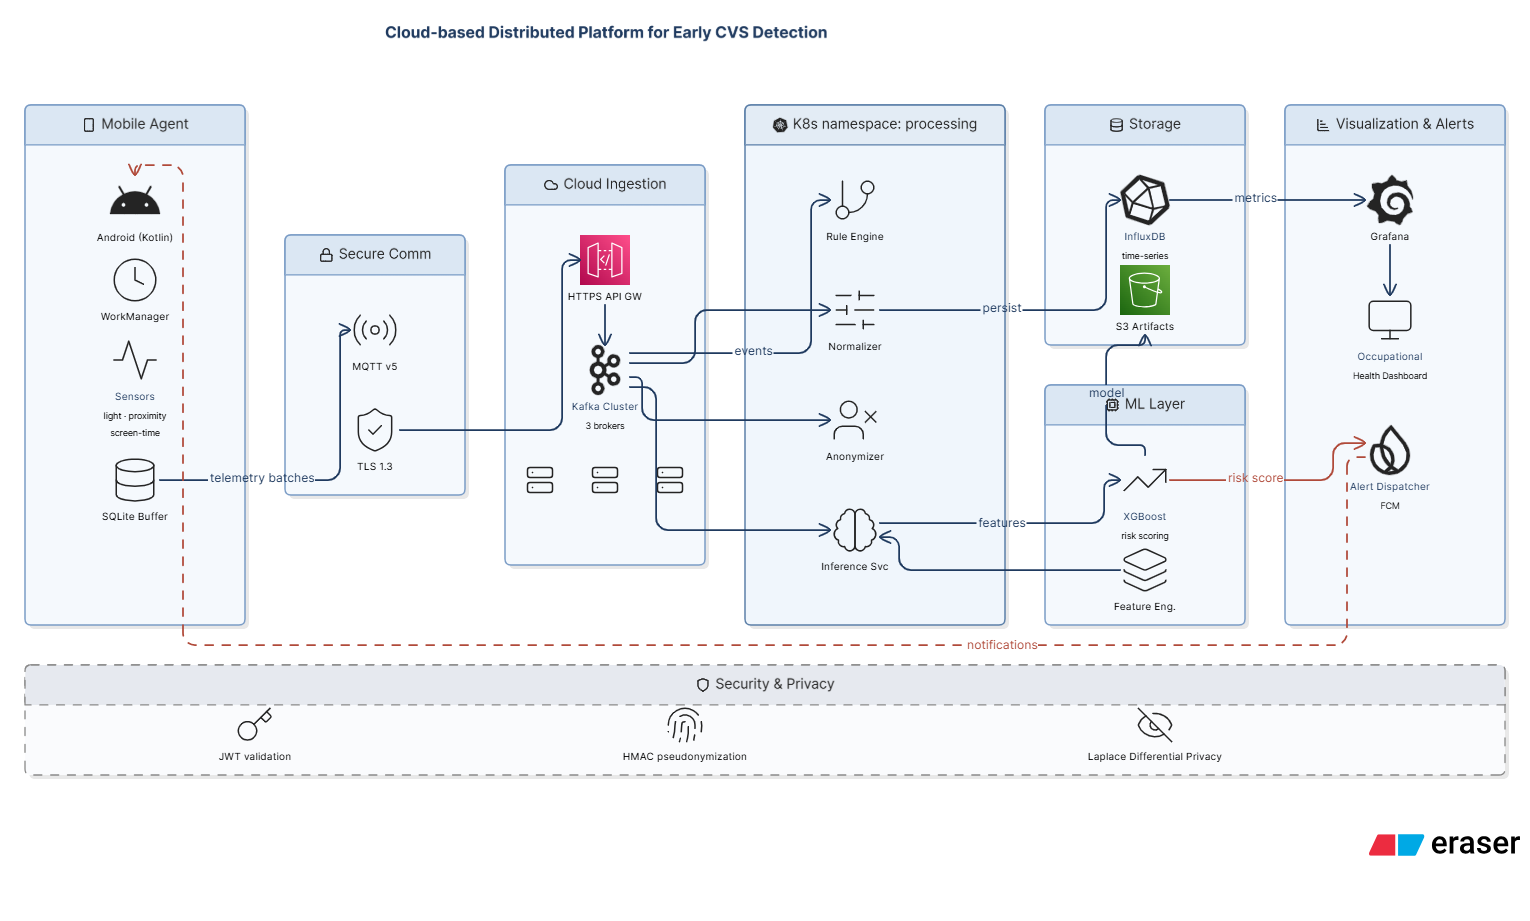
\includegraphics[width=\linewidth]{arch_highlevel.png}
  \caption{Vista general de la plataforma. La figura representa el
           diseño objetivo; la composición que efectivamente corre
           hoy se describe en la sección~\ref{sec:prototipo}.}
  \label{fig:vista-general}
\end{figure}

\FloatBarrier
\section{Arquitectura}\label{sec:arquitectura}

\subsection{Vista detallada}

El topic principal de Kafka es el de telemetría cruda. En el diseño 
objetivo, pensado para una infraestructura administrada con tres 
brokers y hasta 10.000 dispositivos concurrentes, tiene 12 particiones 
y factor de replicación 3. En el prototipo local los tópicos se 
autocrean con particiones por defecto.

Los microservicios siguen un esquema de consumidor compartido 
(figura~\ref{fig:flujo}). El rule engine evalúa reglas duras: sesión 
continua mayor a 45 minutos sin pausa, distancia menor a 30~cm 
sostenida más de cinco minutos, y mismatch de luz ambiente. Cuando 
alguna se rompe, publica una alerta y sigue. En paralelo, el 
normalizer estandariza los valores por modalidad de sensor, y el 
anonymizer cambia el identificador por su seudónimo y aplica ruido de 
Laplace a los valores continuos. El resultado se escribe en InfluxDB.

\begin{figure}[!ht]
  \centering
  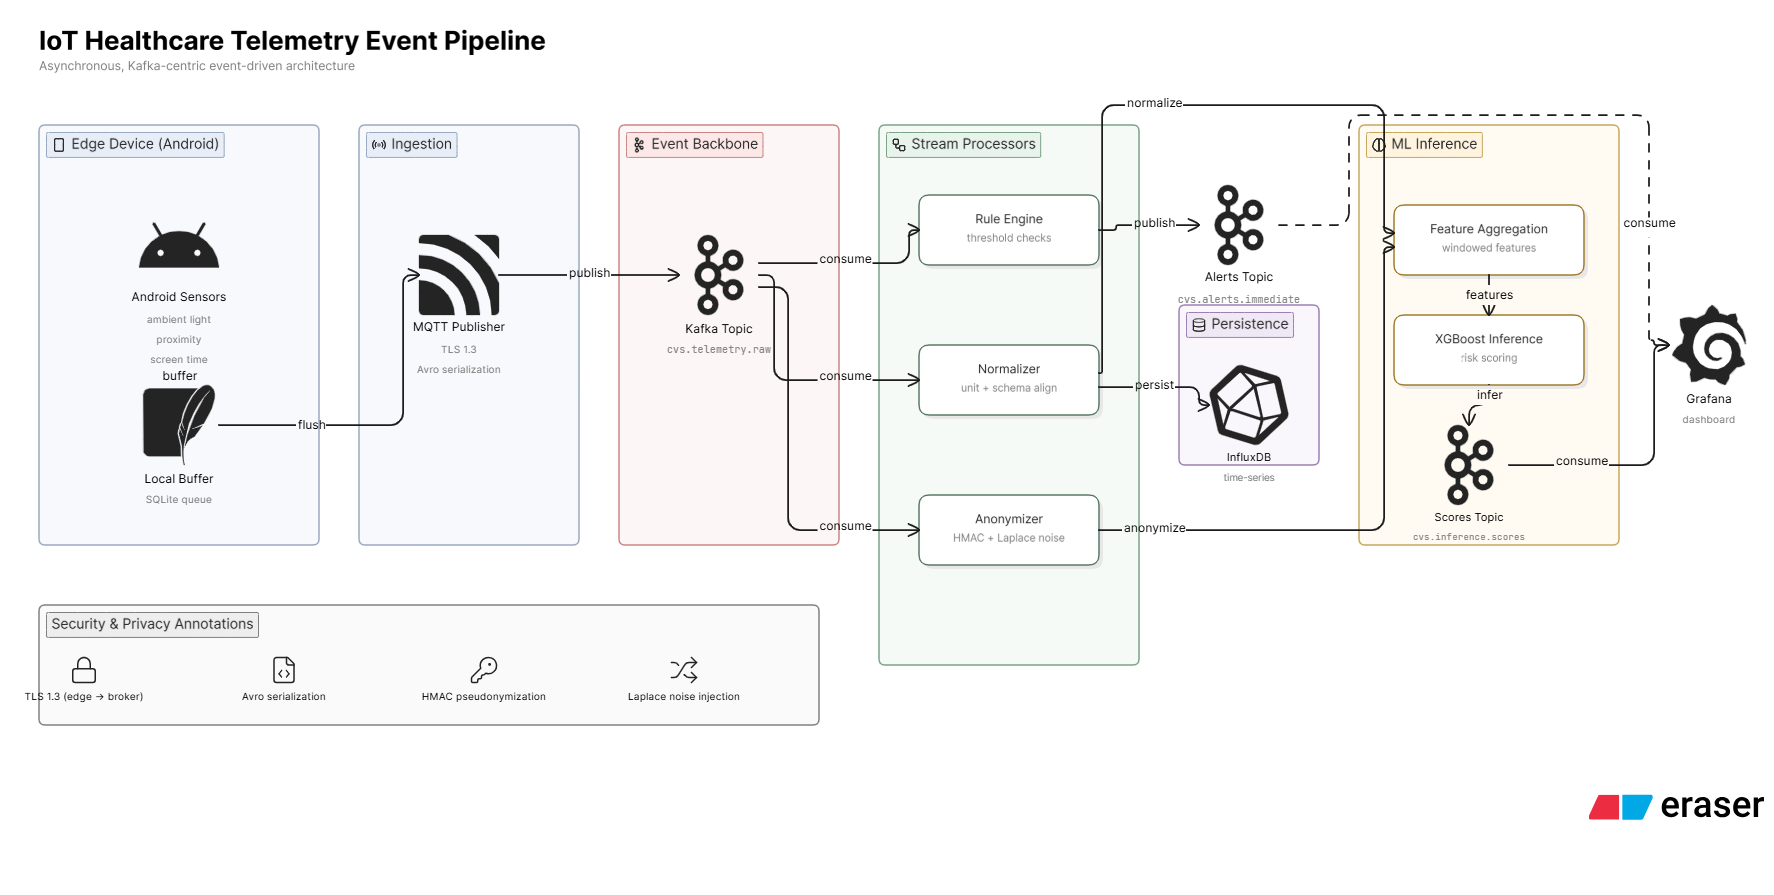
\includegraphics[width=\linewidth]{arch_dataflow.png}
  \caption{Pipeline asíncrono de un lote de telemetría. El lado
           izquierdo es el dispositivo. En el centro, el ingreso y
           el topic Kafka. Tres consumidores derivan tres rutas:
           el rule engine hacia las alertas inmediatas, el normalizer
           y el anonymizer hacia InfluxDB, y la inferencia consume
           del modelo y publica los puntajes.}
  \label{fig:flujo}
\end{figure}

El servicio de inferencia, separado de esa cadena, lee ventanas de 30 
días por usuario seudonimizado, calcula nueve variables agregadas 
(medias, desviaciones y conteos de pausas) y aplica el modelo XGBoost. 
El resultado, un puntaje en $[0,1]$, queda disponible vía un endpoint 
REST.

\subsection{Tópicos de Kafka}

La tabla~\ref{tab:topics} documenta los cuatro tópicos del camino de 
datos en la configuración objetivo.

\begin{table}[H]
  \centering
  \caption{Tópicos de Kafka. Las particiones y la replicación corresponden
           al diseño objetivo para infraestructura administrada;
           el prototipo local usa un broker y particiones por defecto.}
  \label{tab:topics}
  \begin{tabularx}{\linewidth}{@{}p{3.5cm} c c X@{}}
    \toprule
    Tópico & Part. & Repl. & Propósito \\
    \midrule
    cvs.telemetry.raw        & 12 & 3 & Lotes recién recibidos del agente \\
    cvs.telemetry.normalized & 12 & 3 & Lecturas estandarizadas y anonimizadas \\
    cvs.alerts.immediate     &  6 & 3 & Violaciones a reglas duras \\
    cvs.inference.scores     &  6 & 3 & Puntajes de riesgo por usuario \\
    \bottomrule
  \end{tabularx}
\end{table}

\subsection{Modelo de datos en InfluxDB}

InfluxDB organiza la información en \emph{measurements} con etiquetas 
indexables y campos no indexables. El esquema que usamos para las 
lecturas de los sensores es el de la tabla~\ref{tab:influx}.

\begin{table}[H]
  \centering
  \caption{Esquema de las lecturas de sensores en InfluxDB.}
  \label{tab:influx}
  \begin{tabularx}{\linewidth}{@{}p{1.2cm} p{2.5cm} X@{}}
    \toprule
    Tipo & Nombre & Descripción \\
    \midrule
    Tag   & device\_uuid  & Seudónimo HMAC del dispositivo \\
    Tag   & org\_unit     & Hash de la unidad organizacional \\
    Tag   & sensor\_type  & Luz, proximidad, tiempo \\
    Field & raw\_value    & Lectura original \\
    Field & noised\_value & Valor con ruido Laplace ($\varepsilon=1$) \\
    Field & quality\_flag & 0 OK, 1 interpolado, 2 fuera de rango \\
    \bottomrule
  \end{tabularx}
\end{table}

\subsection{Vista de despliegue}

El despliegue objetivo sobre AWS contempla tres namespaces de 
Kubernetes (ingreso, procesamiento, datos y modelo), Amazon MSK como 
broker administrado, CloudFront, WAF, ALB para el tráfico de entrada, 
Cognito para autenticación, S3 para los artefactos del modelo y KMS 
para cifrado en reposo. La separación en namespaces es operacional: 
permite asignar permisos RBAC distintos a cada equipo (DevOps, datos, 
ML). La figura~\ref{fig:deploy} muestra esa arquitectura.

El prototipo, sin embargo, corre sobre docker compose: un broker 
Kafka en modo KRaft, una instancia de InfluxDB, los cuatro 
microservicios, Prometheus y Grafana. La razón de no haber desplegado 
en AWS está documentada en la sección~\ref{sec:discusion}.

\begin{figure}[!ht]
  \centering
  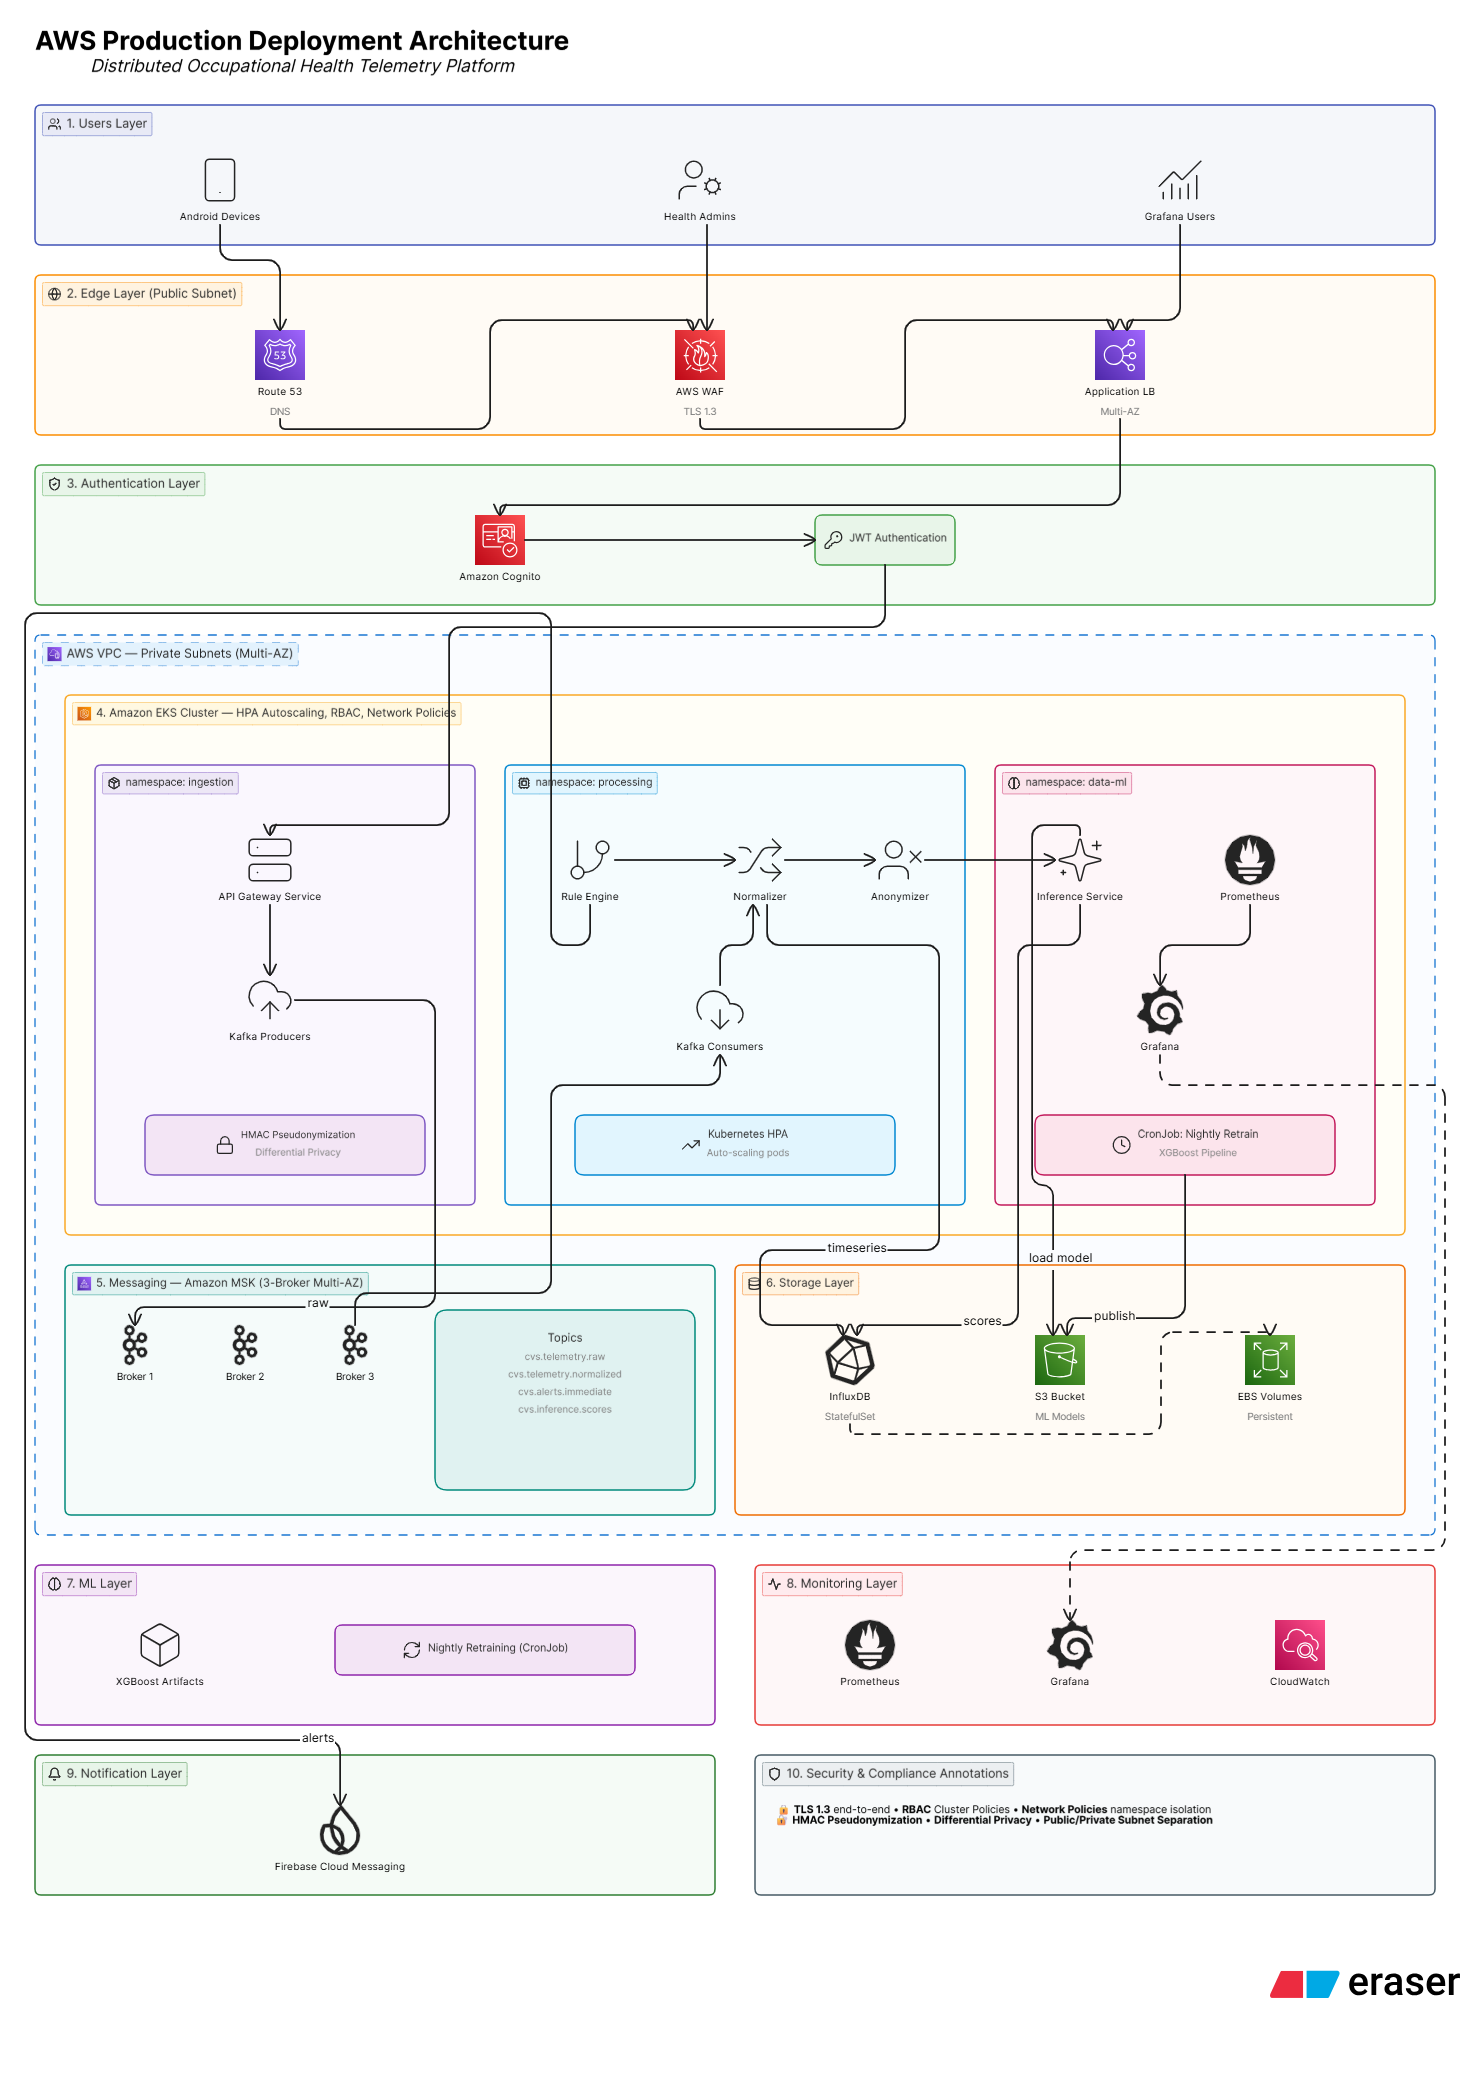
\includegraphics[width=0.92\linewidth]{arch_aws.png}
  \caption{Despliegue de producción sobre AWS como diseño objetivo.
           El tráfico entra por CloudFront, pasa por WAF y ALB, y
           llega al clúster EKS. Cognito y JWT manejan la
           autenticación. Amazon MSK provee el backbone de eventos
           y S3 versiona los artefactos del modelo. Esta arquitectura
           no está desplegada hoy (sección~\ref{sec:discusion}).}
  \label{fig:deploy}
\end{figure}

\subsection{Secuencia de un lote de telemetría}

La figura~\ref{fig:seq} muestra la secuencia que sigue un lote desde 
que el agente lo arma hasta que termina como un puntaje en el 
tablero. Quedan explícitos los dos puntos donde el sistema decide: 
la validación del token de autenticación en el ingreso y la 
bifurcación hacia alerta inmediata cuando se rompe una regla dura.

\begin{figure}[!ht]
  \centering
  \resizebox{0.78\linewidth}{!}{%
  \begin{tikzpicture}[font=\scriptsize,
    msg/.style={-{Stealth[length=2mm]}, thick},
    msgr/.style={-{Stealth[length=2mm]}, thick, red!70!black},
    rret/.style={-{Stealth[length=2mm]}, thick, dashed},
    actor/.style={draw, fill=blue!12, rounded corners,
                  text width=1.55cm, align=center,
                  minimum height=0.55cm, inner sep=2pt,
                  font=\scriptsize\bfseries}]

    \node[actor] (a) at (0,0)   {Agente};
    \node[actor] (b) at (1.9,0) {API\\HTTPS};
    \node[actor] (c) at (3.8,0) {Kafka};
    \node[actor] (d) at (5.7,0) {Rule\\Engine};
    \node[actor] (e) at (7.6,0) {Norm.\\+ Anon.};
    \node[actor] (f) at (9.5,0) {InfluxDB};

    \foreach \x in {0,1.9,3.8,5.7,7.6,9.5}
      \draw[dashed, gray!70] (\x,-0.3) -- (\x,-6.4);

    \fill[blue!25] (-0.07,-0.7) rectangle (0.07,-6.0);
    \fill[blue!25] (1.83,-0.7) rectangle (1.97,-1.4);
    \fill[orange!35] (5.63,-1.7) rectangle (5.77,-2.7);
    \fill[orange!35] (7.53,-3.2) rectangle (7.67,-4.7);
    \fill[violet!30] (9.43,-4.6) rectangle (9.57,-5.3);

    \draw[msg] (0,-0.85)  -- node[above]{1: POST /v1/telemetry} (1.9,-0.85);
    \draw[msg] (1.9,-1.25)-- node[above]{2: validate(JWT)} (3.8,-1.25);
    \draw[msg] (3.8,-1.85)-- node[above]{3: consume(raw)} (5.7,-1.85);

    \draw[red!60!black, thick] (5.4,-2.05) rectangle (8.0,-2.95);
    \node[font=\tiny\bfseries, text=red!60!black, anchor=west] at (5.4,-2.05) {alt: regla rota?};
    \draw[msgr] (5.7,-2.45) -- node[above,font=\tiny]{publish(alert)} (3.8,-2.45);
    \draw[msgr] (3.8,-2.75) -- node[above,font=\tiny]{push FCM} (0,-2.75);

    \draw[msg] (5.7,-3.35) -- node[above]{4: forward(ok)} (7.6,-3.35);
    \draw[msg] (7.6,-3.85)
      .. controls (8.4,-3.85) and (8.4,-4.20) ..
      node[right, font=\tiny] {HMAC + DP} (7.6,-4.20);
    \draw[msg] (7.6,-4.40) -- node[above]{5: write(point)} (9.5,-4.40);

    \draw[rret] (1.9,-5.7) -- node[above]{202 Accepted} (0,-5.7);
  \end{tikzpicture}%
  }
  \caption{Diagrama de secuencia. El bloque \emph{alt} marca la
           bifurcación a alerta inmediata cuando una regla dura se
           rompe.}
  \label{fig:seq}
\end{figure}

\subsection{Seguridad}

La seguridad se manejó por capas. En el prototipo están activos tres 
mecanismos: la seudonimización HMAC del identificador del dispositivo 
antes de escribir a InfluxDB, el ruido de Laplace ($\varepsilon=1$) 
sobre las lecturas continuas, y la validación del contrato de los 
lotes recibidos, que rechaza cualquiera que no traiga un hash de 
consentimiento.

En el diseño objetivo se contempla además validación JWT en el 
ingreso vía Cognito, TLS extremo a extremo entre servicios, WAF en 
el borde, cifrado de la base local del agente y políticas de red 
estrictas entre namespaces. Esos mecanismos están descritos en la 
arquitectura pero no implementados en la versión que corre hoy.

\begin{figure}[!ht]
  \centering
  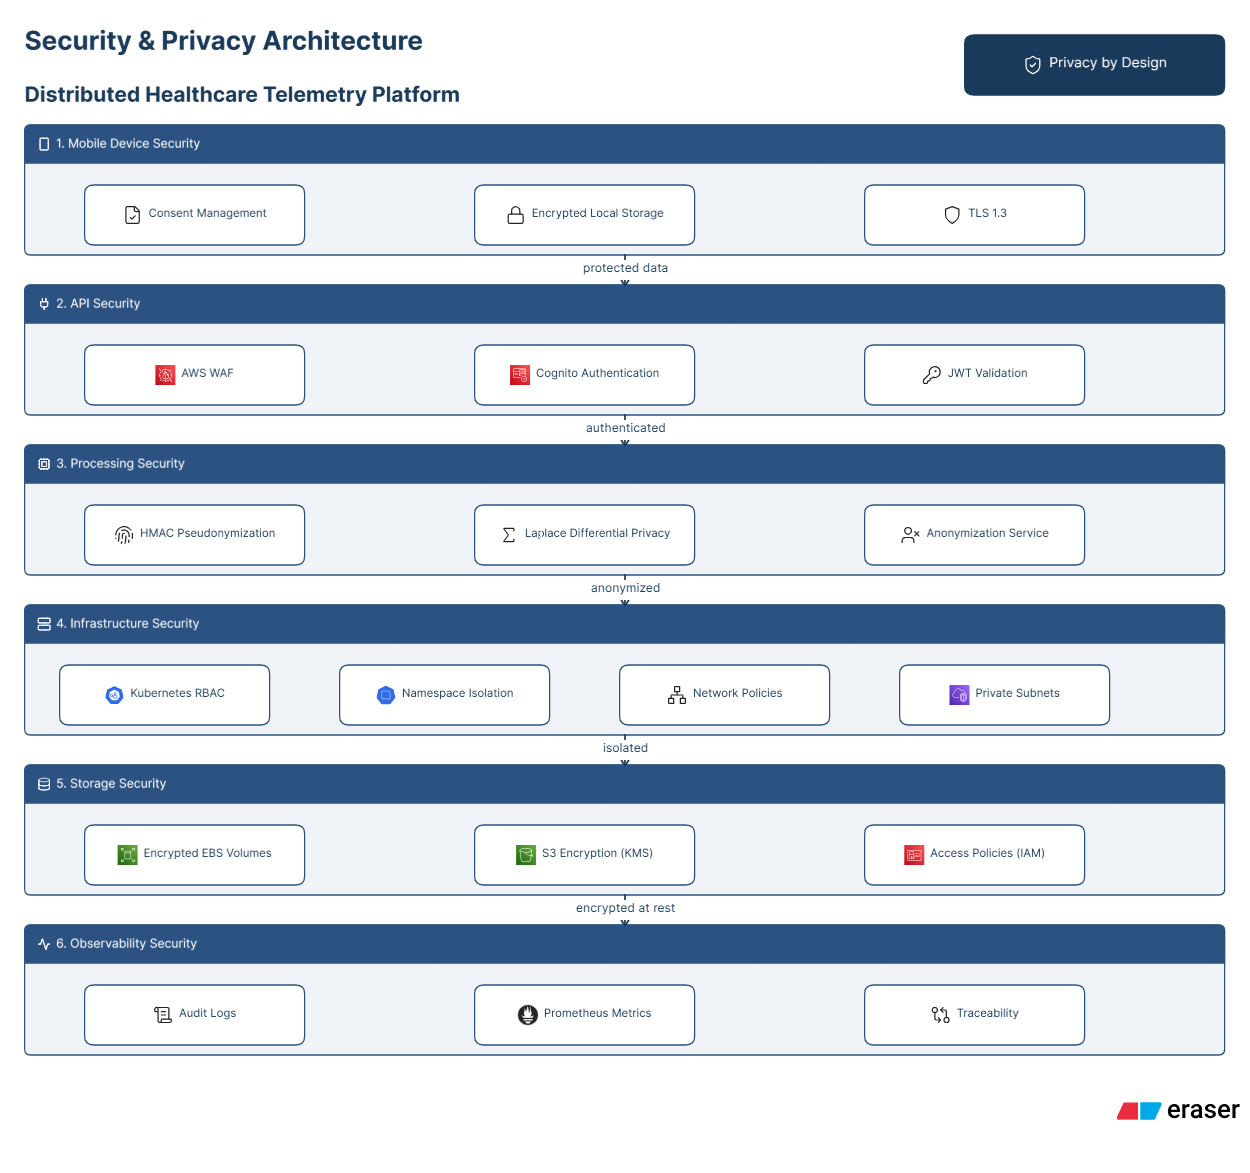
\includegraphics[width=0.72\linewidth]{arch_security.png}
  \caption{Modelo de seguridad por capas como diseño objetivo. En
           el prototipo solo están activas las capas de procesamiento
           (HMAC y Laplace) y el contrato de consentimiento.}
  \label{fig:seguridad}
\end{figure}

\FloatBarrier
\section{Prototipo}\label{sec:prototipo}

\subsection{Stack tecnológico}

\begin{table}[H]
  \centering
  \caption{Stack del prototipo.}
  \label{tab:stack}
  \begin{tabularx}{\linewidth}{@{}>{\bfseries}p{2.4cm} X@{}}
    \toprule
    Capa & Tecnología y motivo \\
    \midrule
    Agente Android & Kotlin con WorkManager y Room. Código presente,
              no desplegado en dispositivos físicos durante el curso. \\
    Transporte & Cliente MQTT en el agente. El prototipo local
              no incluye broker MQTT; la ingestión se hace vía HTTP
              REST contra el servicio de inferencia. \\
    Mensajería & Apache Kafka 7.6.1 (Confluent) en modo KRaft, un solo
              broker. \\
    Servicios & Python 3.11 con FastAPI. Cuatro servicios:
              rule engine, normalizer, anonymizer e inference. \\
    Persistencia & InfluxDB 2.7. \\
    Modelo ML & XGBoost 2.0 entrenado sobre el dataset sintético. \\
    Empaquetado & docker compose en el prototipo;
              Helm 3 y Terraform escritos pero no aplicados. \\
    Tableros & Grafana 10.4 con tres dashboards esqueleto. \\
    \bottomrule
  \end{tabularx}
\end{table}

\subsection{Agente móvil}

El agente está implementado en Kotlin sobre WorkManager. Un worker se 
programa cada 30 segundos y delega en tres colectores (luz, 
proximidad, tiempo activo) que persisten las lecturas en una base 
local con Room. Un segundo worker, cada cinco minutos, arma el lote 
y lo publica vía MQTT. El consentimiento del usuario se gestiona 
explícitamente: solo después de aceptarlo arranca la cadena de 
workers.

WorkManager fue una elección consciente. Habríamos podido usar un 
foreground service con hilo propio, pero eso obliga a mostrar una 
notificación permanente en la barra de estado, lo que estresa a los 
usuarios. WorkManager se acopla bien con el modo de ahorro agresivo 
de Android y agenda el trabajo en ventanas de oportunidad sin 
servicio en primer plano. El precio es que la frecuencia mínima 
garantizada es de 15 minutos; por eso programamos las muestras de 
30 segundos como peticiones de una sola vez que se reencolan a sí 
mismas.

El agente tiene tres limitaciones conocidas: no se probó en 
dispositivos físicos durante el curso, solo a nivel de código y 
unit tests; el cifrado de la base local con SQLCipher no quedó 
operativo; y como no hay broker MQTT en la composición local, no 
validamos extremo a extremo el camino agente $\rightarrow$ MQTT 
$\rightarrow$ Kafka.

\subsection{Microservicios en Python}

Los cuatro servicios exponen endpoints de health y métricas para 
Prometheus, y arrancan un hilo consumidor de Kafka al inicializar. 
El rule engine implementa las tres reglas duras: sesión continua de 
más de 45 minutos sin pausa, proximidad menor a 20~cm sostenida y 
mismatch de iluminación ambiente. El normalizer aplica z-score por 
sensor. El anonymizer aplica HMAC-SHA256 truncado a 32 caracteres 
hexadecimales más ruido de Laplace por sensor, y rechaza cualquier 
lote sin hash de consentimiento. El servicio de inferencia extrae 
las variables agregadas del lote y delega en el scorer; mantiene un 
cache en memoria por dispositivo, y si el modelo no está cargado 
devuelve un error 503.

\subsection{Esquema de mensajes}

Definimos el contrato de los lotes como un esquema Avro y lo 
mantenemos en el repositorio para que sirva como referencia 
evolutiva, pero el prototipo deserializa los lotes como JSON. 
Migrar a Avro en runtime es trabajo pendiente.

\begin{lstlisting}[language=json, caption={Esquema Avro del lote
  de telemetría (contrato evolutivo).},
  basicstyle=\ttfamily\scriptsize]
{
  "type": "record",
  "name": "TelemetryBatch",
  "namespace": "edu.escuelaing.cvs",
  "fields": [
    {"name": "device_uuid", "type": "string"},
    {"name": "batch_timestamp", "type": "long"},
    {"name": "readings", "type": {
      "type": "array",
      "items": {
        "type": "record",
        "name": "SensorReading",
        "fields": [
          {"name": "sensor_type", "type": {
            "type": "enum", "name": "SensorType",
            "symbols": ["AMBIENT_LIGHT","PROXIMITY","SCREEN_TIME"]}},
          {"name": "value", "type": "float"},
          {"name": "sampled_at", "type": "long"}]}}},
    {"name": "consent_hash", "type": "string"}
  ]
}
\end{lstlisting}

\subsection{Privacidad: HMAC y ruido de Laplace}

La pieza de privacidad tiene dos partes. La seudonimización deriva 
un identificador determinista a partir del UUID del dispositivo y 
una llave del operador, mediante HMAC-SHA256. La función es la 
misma en cualquier réplica del servicio, lo cual permite agrupar 
por usuario en la base sin saber quién es. La segunda parte aplica 
ruido aleatorio con distribución de Laplace a los valores 
continuos, calibrado por un parámetro $\varepsilon$ que controla 
cuánto se distorsionan los valores:

\begin{lstlisting}[language=Python,
  caption={Mecanismo de Laplace usado para perturbar lecturas
           continuas.},
  basicstyle=\ttfamily\scriptsize]
import numpy as np

def add_laplace_noise(value: float,
                      epsilon: float = 1.0,
                      sensitivity: float = 1.0) -> float:
    if epsilon <= 0:
        raise ValueError("epsilon debe ser positivo")
    scale = sensitivity / epsilon
    return float(value + np.random.laplace(0.0, scale))
\end{lstlisting}

El ruido tiene un costo medible en la utilidad de las lecturas 
individuales, pero ese costo se diluye al agregar miles de 
lecturas. La auditoría reportada en la sección~\ref{sec:resultados} 
verifica que el ruido no rompe la distribución a nivel agregado.

\subsection{Pipeline de aprendizaje automático}

El generador del dataset produce 50.000 registros día-usuario 
etiquetados con una regla simple sobre cumplimiento de pausas y 
duración máxima de sesión, alineada con los umbrales de Sheppard y 
Wolffsohn~\cite{sheppard2018}. El entrenamiento corre con XGBoost 
en validación cruzada de cinco folds y rechaza el modelo si F1 cae 
por debajo de 0,75 o AUC por debajo de 0,80. El artefacto validado 
se sube a S3 con un puntero a la versión más reciente. El 
entrenamiento nocturno se dispara desde GitHub Actions.

\begin{figure}[!ht]
  \centering
  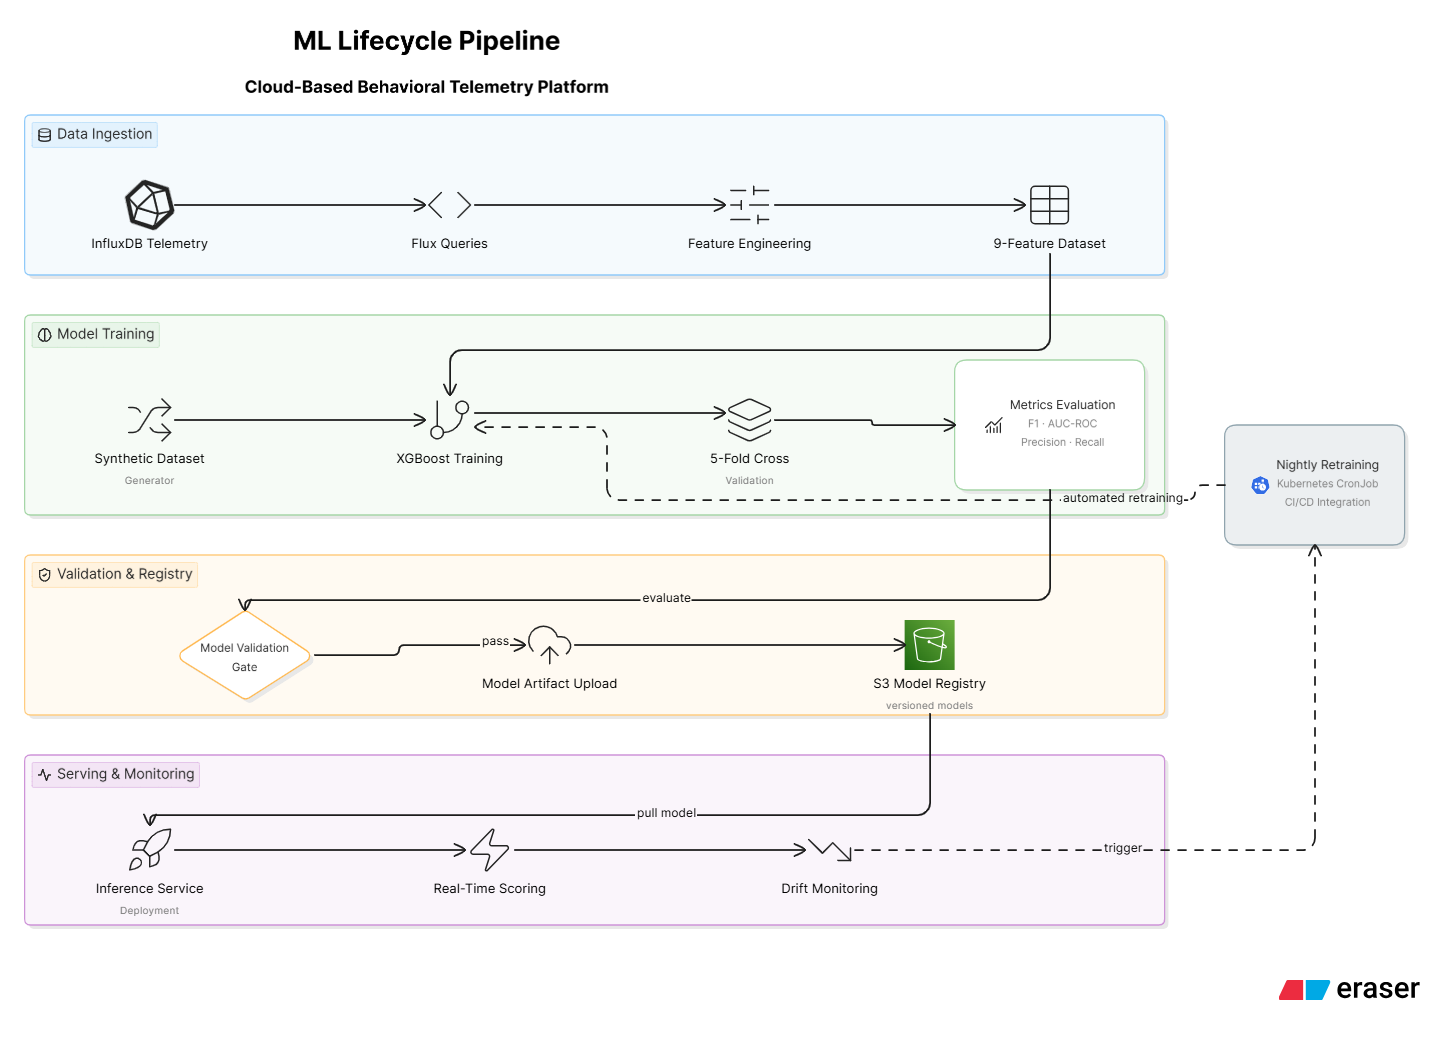
\includegraphics[width=\linewidth]{arch_ml.png}
  \caption{Ciclo de vida del modelo: ingesta del dataset, entrenamiento
           con validación cruzada, gate de validación que rechaza
           modelos por debajo de los umbrales, registro en S3, y
           carga por el servicio de inferencia.}
  \label{fig:ml}
\end{figure}

\subsection{Despliegue}

Cada microservicio tiene un chart de Helm con plantillas estándar 
de Kubernetes (Deployment, Service, HPA, ConfigMap y 
ServiceMonitor). El HPA está configurado al 70\,\% de uso de CPU, 
valor consistente con la recomendación oficial para servicios 
\emph{stateless}~\cite{kubernetes}. El ServiceMonitor requiere 
Prometheus Operator instalado; en el prototipo local Prometheus 
hace scrape estático.

La infraestructura como código contempla módulos Terraform para 
EKS, MSK y S3, pero el Terraform no se aplicó. Hay dos razones. La 
primera es que la cuenta AWS asignada al curso es un AWS Academy 
Learner Lab, que aplica una política administrada denegando la 
creación de roles IAM, clústers EKS y clústers MSK. La segunda es 
que los módulos contienen identificadores de VPC y subred como 
placeholders, así que aún en una cuenta sin restricciones habría 
que sustituirlos.

El prototipo corre sobre docker compose, que levanta los mismos 
componentes lógicos del diagrama de despliegue (Kafka, InfluxDB, 
los cuatro microservicios, Prometheus y Grafana) con las mismas 
imágenes y puertos. La diferencia con AWS es la capa de 
infraestructura: un solo broker en lugar de tres, sin balanceador 
de carga, sin Cognito. El camino del dato a nivel lógico es el 
mismo.

\subsection{Integración continua}

El repositorio tiene cuatro workflows en GitHub Actions: uno de 
integración continua que corre linter, type checker y tests con 
cobertura sobre cada PR; dos workflows de despliegue (staging y 
producción) que están escritos como plantilla pero apuntan a 
clústers que no aprovisionamos; y un workflow nocturno para el 
entrenamiento del modelo. El workflow de CI bloquea el merge si la 
cobertura cae por debajo del 80\,\% en código nuevo.

\FloatBarrier
\section{Resultados}\label{sec:resultados}

\subsection{Modelo XGBoost sobre dataset sintético}

Antes de entrenar revisamos las distribuciones de las nueve 
variables sobre los 50.000 registros (figura~\ref{fig:dataset}). La 
inspección visual confirmó que los rangos caen donde esperábamos 
según la literatura clínica (lux entre 20 y 1500, distancia entre 
18 y 90~cm, sesiones continuas entre 15 y 180~min) y nos alertó de 
que la cola larga del tiempo de pantalla (usuarios con 14 a 15 
horas al día) es poco realista. Ese ajuste lo haríamos cuando 
lleguen los primeros datos reales del estudio piloto.

\begin{figure}[!ht]
  \centering
  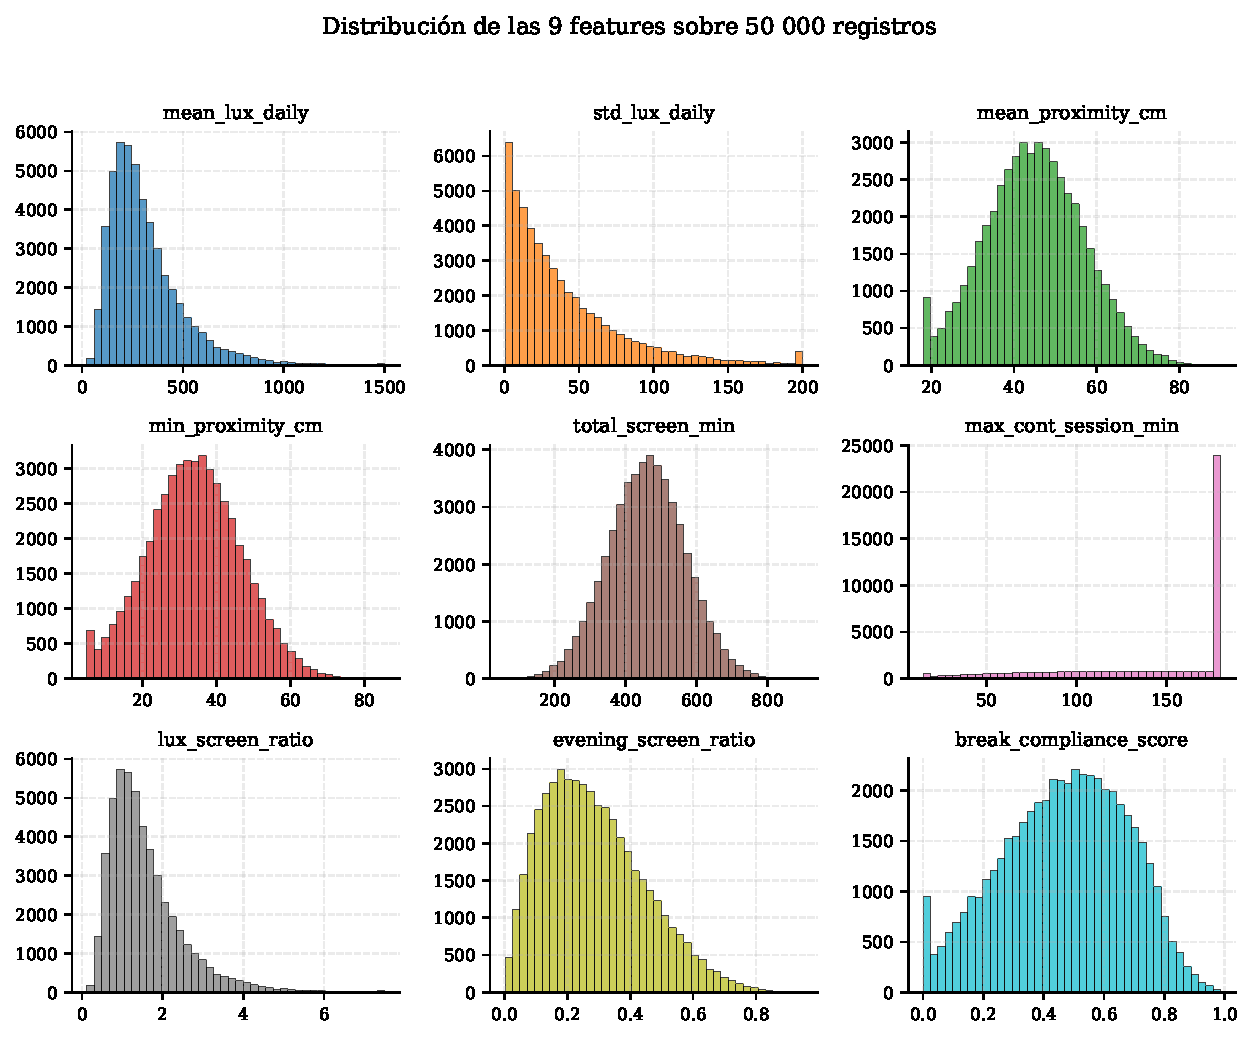
\includegraphics[width=0.95\linewidth]{dataset_overview.pdf}
  \caption{Distribución empírica de las nueve variables del
           dataset sintético. 50.000 registros usuario-día.}
  \label{fig:dataset}
\end{figure}

Sobre ese dataset, dividido 80/20 con estratificación y validación 
cruzada de cinco folds sobre el conjunto de entrenamiento, el 
modelo dio los resultados de la tabla~\ref{tab:ml}.

\begin{table}[H]
  \centering
  \caption{Métricas del clasificador. CV: validación cruzada de cinco
    folds sobre entrenamiento. Test: 10.000 registros del holdout.}
  \label{tab:ml}
  \begin{tabular}{@{}lcccc@{}}
    \toprule
    Conjunto & F1 macro & AUC-ROC & Precisión & Exhaustividad \\
    \midrule
    CV (mean) & 0,853 & 0,892 & 0,858 & 0,849 \\
    CV (std)  & 0,004 & 0,003 & 0,004 & 0,004 \\
    Test      & 0,854 & 0,894 & 0,864 & 0,849 \\
    \bottomrule
  \end{tabular}
\end{table}

\begin{figure}[!ht]
  \centering
  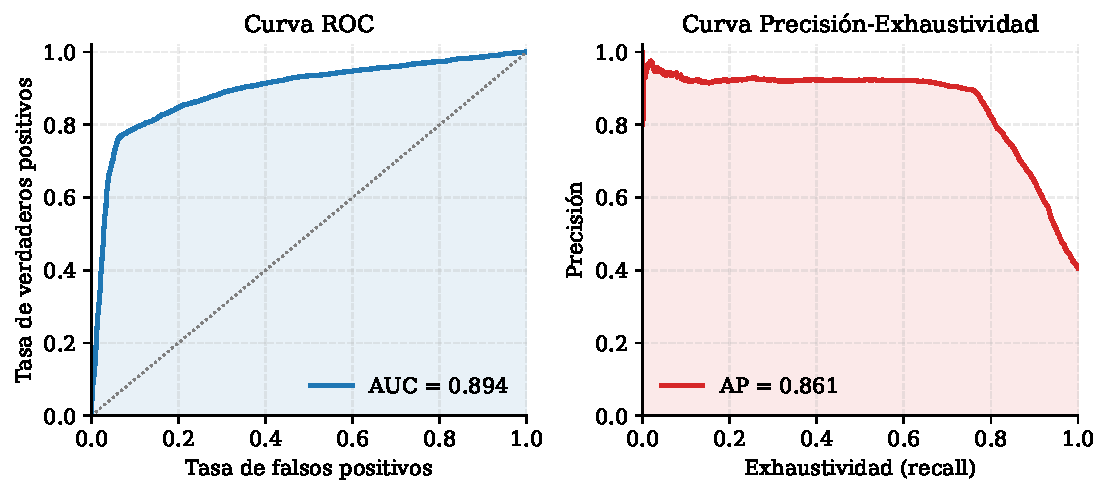
\includegraphics[width=\linewidth]{roc_curve.pdf}
  \caption{Curva ROC (AUC = 0{,}894) y curva
           precisión-exhaustividad (AP = 0{,}872) sobre el holdout
           (10.000 registros).}
  \label{fig:roc}
\end{figure}

La importancia que XGBoost asigna a cada variable 
(figura~\ref{fig:featimp}) tiene una observación importante. Las 
dos más altas, el cumplimiento de pausas y la duración máxima de 
sesión, son los componentes literales de la regla de etiquetado, 
así que eran lo esperado. La tercera, la proximidad mínima al 
rostro, no entra en la regla y aun así aparece arriba: el modelo 
está usando información ergonómica adicional para refinar su 
predicción. Eso encaja con la literatura clínica que liga la 
distancia mínima al rostro con el esfuerzo de 
acomodación~\cite{blehm2005}.

\begin{figure}[!ht]
  \centering
  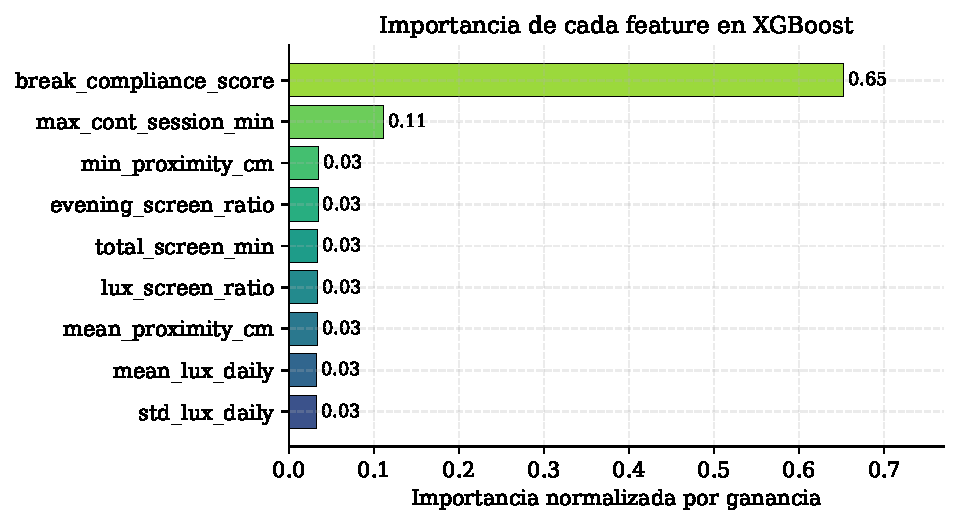
\includegraphics[width=0.92\linewidth]{feature_importance.pdf}
  \caption{Importancia de las nueve variables en XGBoost.}
  \label{fig:featimp}
\end{figure}

\begin{figure}[!ht]
  \centering
  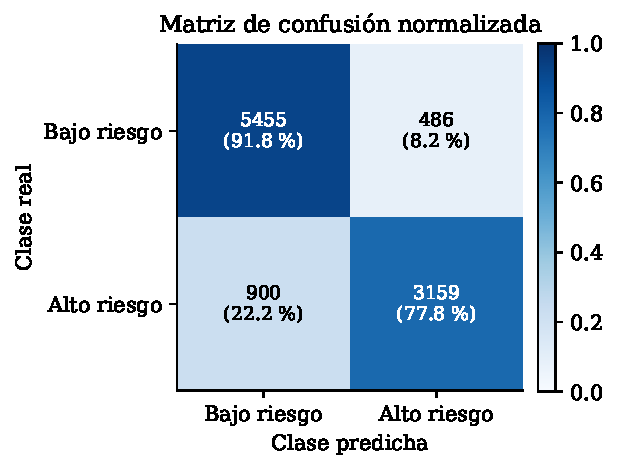
\includegraphics[width=0.43\linewidth]{confusion_matrix.pdf}
  \caption{Matriz de confusión normalizada sobre el holdout.}
  \label{fig:cm}
\end{figure}

Una aclaración importante sobre estos números. Las dos variables 
más importantes son los componentes literales de la regla de 
etiquetado, así que el F1 de 0,85 no es un resultado clínico: es 
la capacidad del modelo de recuperar la regla con la que se 
etiquetaron los datos. Es útil para validar que la cadena de 
entrenamiento funciona, pero no es evidencia de detección de CVS 
en humanos. Esa validación es trabajo futuro.

\subsection{Smoke test extremo a extremo}

Para asegurarnos de que la cadena completa funciona, hicimos un 
script que levanta la composición completa, envía un lote real con 
tres lecturas (luz, proximidad, tiempo de pantalla) al endpoint de 
ingesta y verifica que el endpoint de puntaje responda con un 
valor en $[0,1]$ y un nivel cualitativo (LOW, MEDIUM o HIGH). El 
script también hace health check de los cuatro servicios.

Cuando corre contra docker compose en local, los cuatro health 
endpoints responden 200, el POST devuelve 202, y una vez el modelo 
está cargado, el GET devuelve el puntaje. Eso confirma que el 
camino feliz funciona en la composición local.

\subsection{Auditoría de privacidad}

Una segunda suite de pruebas, todas offline, verifica las 
propiedades de los mecanismos de privacidad. Son cinco pruebas: un 
test de Kolmogorov-Smirnov sobre 10.000 muestras del ruido Laplace 
generado, frente a la distribución teórica; verificación del 
formato del seudónimo HMAC (32 caracteres hexadecimales); 
determinismo del HMAC (la misma entrada produce el mismo 
seudónimo); validación del contrato de los lotes anonimizados, que 
rechaza cualquiera que no traiga hash de consentimiento; e 
inspección del protocolo de escritura a InfluxDB, que verifica que 
las líneas escritas nunca contienen el UUID crudo. Las cinco 
pasan con $\varepsilon = 1$. Es la evidencia de privacidad más 
fuerte del proyecto.

\subsection{Lo que no medimos en esta entrega}

El alcance del prototipo no incluye latencia bajo carga (existe un 
plan de pruebas en JMeter con 50 hilos concurrentes y 500 lotes, 
pero no conservamos un artefacto de salida con percentiles 
defendibles), prueba de escala (no probamos con 10.000 
dispositivos), latencia del endpoint de inferencia bajo carga, 
medición cuantitativa del costo del ruido sobre la utilidad ni 
validación clínica de ningún tipo.

\FloatBarrier
\section{Atributos de calidad}\label{sec:calidad}

\begin{table*}[t]
  \centering
  \small
  \caption{Atributos, SLO objetivo y estado sobre el prototipo.}
  \label{tab:slos}
  \begin{tabularx}{\textwidth}{@{}>{\bfseries}p{2.6cm} p{4cm} p{3.5cm} X@{}}
    \toprule
    Atributo & Escenario & SLO objetivo & Estado \\
    \midrule
    Privacidad &
      Ningún identificador crudo escrito en InfluxDB &
      Cero PII cruda &
      Verificado. Cinco de cinco pruebas pasan. \\
    \addlinespace
    Exactitud ML &
      Clasificación de alto riesgo sobre dataset sintético &
      F1 $\geq 0{,}75$ y AUC $\geq 0{,}80$ &
      Cumple sobre sintético: F1 = 0,85, AUC = 0,89. No
      es evidencia clínica. \\
    \addlinespace
    Camino feliz E2E &
      Ingestión $\rightarrow$ puntaje &
      Smoke test PASS &
      Verificado en docker compose. \\
    \addlinespace
    Rendimiento &
      Ingestión bajo 50 dispositivos concurrentes &
      P99 $\leq 500$~ms &
      No medido con artefacto reproducible. \\
    \addlinespace
    Escalabilidad &
      HPA y multi-broker &
      Activos en clúster &
      No aplicado. Charts y Terraform escritos pero no
      desplegados. \\
    \addlinespace
    Latencia de inferencia &
      P99 del endpoint &
      $\leq 100$~ms &
      No medido bajo carga. \\
    \bottomrule
  \end{tabularx}
\end{table*}

Tres atributos verificados, tres pendientes. Otros atributos que 
típicamente aparecen en este tipo de trabajos (mantenibilidad, 
modificabilidad, testeabilidad) no los listamos como SLOs porque 
no se pueden medir con el mismo rigor. La organización del 
repositorio en carpetas disjuntas, los charts independientes por 
microservicio y la cobertura mínima del 80\,\% sobre código nuevo 
son evidencia indirecta de esos atributos.

\subsection{Observabilidad}

Cada microservicio expone un endpoint de métricas integrado con 
Prometheus. Hay tres dashboards de Grafana preparados (operaciones, 
salud organizacional y desempeño del modelo) como esqueletos: las 
consultas están escritas, pero requieren datos sostenidos en 
InfluxDB para verse poblados, cosa que el prototipo solo produce 
durante el smoke test.

\FloatBarrier
\section{Discusión}\label{sec:discusion}

Hay limitaciones del trabajo que vale la pena nombrar.

El modelo se entrenó con etiquetas derivadas de umbrales clínicos. 
Eso permite probar la cadena, pero el F1 de 0,85 no es un resultado 
clínico: es la capacidad del modelo de recuperar la regla con la 
que se etiquetaron los datos. La validación con trabajadores reales 
y un optómetra es indispensable y queda como trabajo futuro.

El contrato de los lotes está definido como Avro y vive en el 
repositorio, pero el prototipo deserializa JSON. La ganancia de 
compactación que ofrece Avro pertenece al diseño objetivo, no a la 
versión que corre hoy.

El agente Android tiene cliente MQTT, pero la composición local 
no incluye broker MQTT ni bridge a Kafka. El camino que validamos 
es HTTP REST contra el servicio de inferencia. El flujo agente 
$\rightarrow$ MQTT $\rightarrow$ Kafka es diseño.

Los módulos Terraform tienen identificadores de VPC y subred como 
placeholders, y la cuenta AWS asignada al curso deniega la creación 
de roles IAM y clústers EKS o MSK. Por las dos razones no aplicamos 
la infraestructura. CloudFront, WAF, ALB, Cognito y KMS aparecen 
en la figura del despliegue como diseño y no como código 
desplegable.

El smoke test envía un encabezado de autorización, pero ningún 
servicio valida el token en el prototipo. La validación JWT con 
Cognito está pensada como diseño objetivo.

El esquema de privacidad oculta el identificador y perturba las 
lecturas, pero no contabiliza el consumo acumulado de $\varepsilon$ 
por usuario. Un despliegue real exigiría llevar ese acumulador, 
en la línea de las técnicas descritas por Dwork y 
Roth~\cite{dwork2014}.

El código del agente compila y tiene tests unitarios, pero no se 
desplegó en un teléfono real durante el curso.

\subsection*{Frente a las herramientas que existen}

Para el trabajador individual la experiencia se parece bastante a 
la de Apple Screen Time o Google Digital Wellbeing: cada cierto 
tiempo le llega un recordatorio de pausa. La diferencia está en el 
otro lado. Apple y Google son aplicaciones que viven en el celular; 
lo nuestro es una plataforma con servidor. Eso permite que un área 
de salud ocupacional vea una distribución por equipo, compare 
departamentos, o detecte que un grupo lleva varias semanas con 
peor cumplimiento de pausas que el resto. Con las herramientas 
comerciales eso no se puede hacer.

Las cuatro líneas de continuación más relevantes son la 
validación clínica con un grupo voluntario y un cuestionario 
estandarizado, el despliegue real de la infraestructura sobre 
una cuenta AWS sin restricciones, la activación de la capa de 
autenticación con JWT en el ingreso, y el endurecimiento del 
canal MQTT desde el agente.
\newpage
\begin{thebibliography}{10}

\bibitem{sheppard2018}
A. L. Sheppard y J. S. Wolffsohn,
``Digital eye strain: prevalence, measurement and amelioration,''
\emph{BMJ Open Ophthalmology}, vol. 3, no. 1, art. e000146, 2018.

\bibitem{blehm2005}
C. Blehm, S. Vishnu, A. Khattak, S. Mitra y R.~W. Yee,
``Computer vision syndrome: a review,''
\emph{Survey of Ophthalmology}, vol. 50, no. 3, pp. 253--262, 2005.

\bibitem{lane2010}
N.~D. Lane, E. Miluzzo, H. Lu, D. Peebles, T. Choudhury y A.~T. Campbell,
``A survey of mobile phone sensing,''
\emph{IEEE Communications Magazine}, vol. 48, no. 9, pp. 140--150, 2010.

\bibitem{aoa2023}
American Optometric Association y Deloitte Economics Institute,
``The Impact of Unmanaged Excessive Screen Time in the United States,''
informe técnico, 2023.

\bibitem{kafka}
Apache Software Foundation,
``Apache Kafka Documentation,'' [En línea]. Disponible:
\url{https://kafka.apache.org/documentation/}

\bibitem{influxdata}
InfluxData,
``InfluxDB OSS v2 Documentation,''
[En línea]. Disponible:
\url{https://docs.influxdata.com/influxdb/v2/}

\bibitem{xgboost}
T. Chen y C. Guestrin,
``XGBoost: A Scalable Tree Boosting System,''
en \emph{Proc. 22nd ACM SIGKDD KDD}, 2016, pp. 785--794.

\bibitem{dwork2014}
C. Dwork y A. Roth,
``The Algorithmic Foundations of Differential Privacy,''
\emph{Foundations and Trends in TCS}, vol. 9, no. 3-4,
pp. 211--407, 2014.

\bibitem{mcmahan2017}
H. B. McMahan, E. Moore, D. Ramage, S. Hampson y B.~A. y~Arcas,
``Communication-Efficient Learning of Deep Networks from
Decentralized Data,'' en \emph{Proc. AISTATS}, vol. 54, 2017,
pp. 1273--1282.

\bibitem{gdpr2016}
Parlamento Europeo y Consejo de la UE,
``Reglamento (UE) 2016/679 — RGPD,'' 2016.

\bibitem{kubernetes}
The Kubernetes Authors,
``Horizontal Pod Autoscaling,'' Kubernetes Documentation, 2024.

\end{thebibliography}

\end{document}